\documentclass[12pt,a4paper]{article}
\usepackage[utf8]{inputenc}
\usepackage[brazil]{babel}
\usepackage{graphicx}
\usepackage{hyperref}
\usepackage{listings}
\usepackage{xcolor}
\usepackage{geometry}

\geometry{margin=2.5cm}

% Configuração de código
\lstset{
    basicstyle=\ttfamily\footnotesize,
    breaklines=true,
    frame=single,
    numbers=left,
    numberstyle=\tiny\color{gray},
    keywordstyle=\color{blue},
    commentstyle=\color{green!60!black},
    stringstyle=\color{red},
    showstringspaces=false,
    tabsize=2,
    backgroundcolor=\color{gray!10}
}

\title{
    \textbf{Trabalho 2: Modelagem e Análise de Dados Legislativos com Neo4j}\\
    \large Banco de Dados para Ciência de Dados
}
\author{
    Guilherme César Athayde - 748175 \\
    \texttt{guilherme.athayde@estudante.ufscar.br}
    \and
    Nome - RA \\
    \texttt{email@estudante.ufscar.br}
}
\date{\today}

\begin{document}

\maketitle
\thispagestyle{empty}

\newpage
\tableofcontents
\newpage

\section{Introdução}

Este trabalho apresenta a modelagem, importação e análise de dados legislativos da Câmara dos Deputados do Brasil utilizando o banco de dados de grafos Neo4j. O objetivo é explorar as relações entre deputados, partidos, proposições e votações para gerar insights sobre o funcionamento do processo legislativo brasileiro.

\subsection{Dataset Escolhido}

O dataset utilizado foi coletado da API de Dados Abertos da Câmara dos Deputados (\url{https://dadosabertos.camara.leg.br}), contendo informações sobre:

\begin{itemize}
    \item \textbf{Deputados}: 513 registros contendo informações sobre parlamentares da 57ª Legislatura (2023-2027), incluindo nome, partido, UF, email e foto.
    \item \textbf{Partidos}: 28 partidos políticos com representação na Câmara, contendo sigla, nome completo e URI de referência.
    \item \textbf{Proposições}: 15 proposições legislativas (PLs, PECs, etc.) com ementa, tipo, número e ano.
    \item \textbf{Votações}: 100 registros de votações realizadas em diferentes órgãos (Plenário, comissões) com descrição, resultado (aprovado/rejeitado) e data.
    \item \textbf{Órgãos}: 8 órgãos legislativos incluindo o Plenário e diversas comissões temáticas.
    \item \textbf{Frentes Parlamentares}: 15 frentes parlamentares temáticas da legislatura atual.
\end{itemize}

Os dados referem-se principalmente ao período de 2023-2025, com foco na legislatura atual e votações recentes (outubro de 2025).

\subsection{Características Importantes do Dataset}

\begin{itemize}
    \item Os dados são estruturados em formato JSON seguindo o padrão da API REST da Câmara.
    \item Existem relacionamentos naturais entre entidades: deputados pertencem a partidos, votações são realizadas por órgãos, proposições podem estar vinculadas a votações.
    \item As descrições de votações frequentemente mencionam nomes de deputados (relatores, autores), permitindo análises textuais.
    \item O campo \texttt{aprovacao} nas votações indica o resultado (1=aprovado, 0=rejeitado, null=outros).
\end{itemize}

\section{Coleta de Dados}

Os dados foram coletados através de requisições HTTP à API de Dados Abertos da Câmara dos Deputados. O script de coleta utiliza \texttt{curl} para fazer as requisições e \texttt{jq} para formatar o JSON de saída.

\subsection{Script de Coleta}

\begin{lstlisting}[language=bash,caption=Script de coleta de dados]
cd datasets
curl -s -H "Content-Type: application/json" \
  https://dadosabertos.camara.leg.br/api/v2/deputados | jq '.' > deputados.json

curl -s -H "Content-Type: application/json" \
  https://dadosabertos.camara.leg.br/api/v2/proposicoes | jq '.' > proposicoes.json

curl -s -H "Content-Type: application/json" -H "Accept: application/json" \
  https://dadosabertos.camara.leg.br/api/v2/votacoes | jq '.' > votacoes.json

curl -s -H "Content-Type: application/json" \
  https://dadosabertos.camara.leg.br/api/v2/orgaos | jq '.' > orgaos.json

curl -s -H "Content-Type: application/json" \
  https://dadosabertos.camara.leg.br/api/v2/partidos | jq '.' > partidos.json

curl -s -H "Content-Type: application/json" \
  https://dadosabertos.camara.leg.br/api/v2/frentes | jq '.' > frentes.json
\end{lstlisting}

\section{Modelagem dos Dados}

A modelagem dos dados em grafo foi projetada para representar as relações naturais entre as entidades do processo legislativo. O diagrama abaixo ilustra o modelo de dados implementado no Neo4j:

\begin{figure}[p]
    \centering
    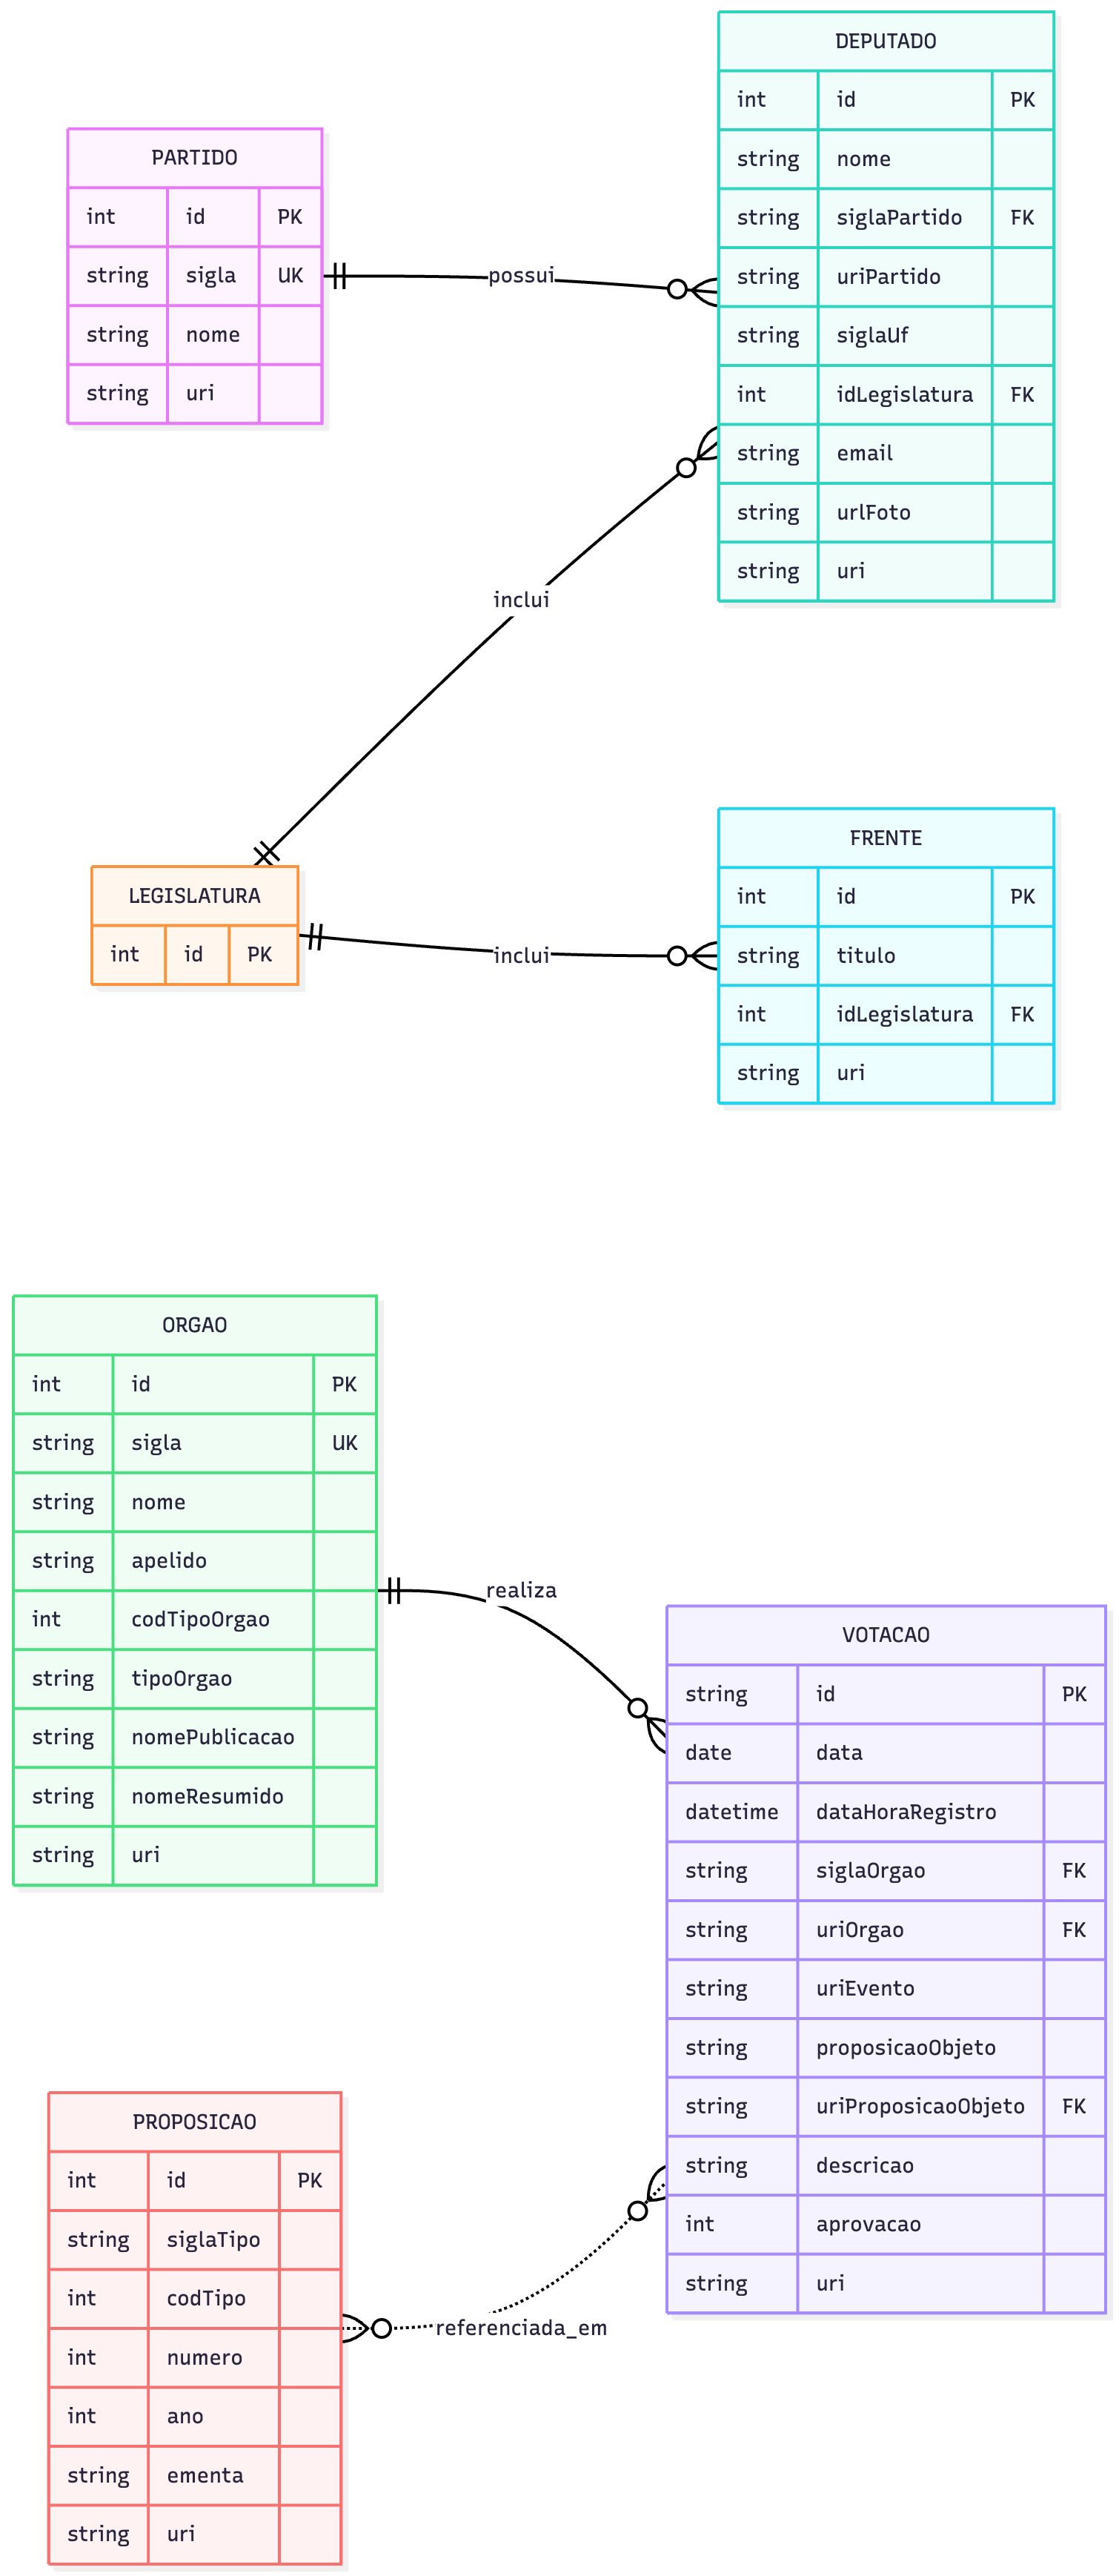
\includegraphics[width=0.85\textwidth,height=0.85\textheight,keepaspectratio]{diagram/Diagram_Mermaid.png}
    \caption{Diagrama do modelo de dados em grafo}
    \label{fig:diagram}
\end{figure}

\subsection{Entidades (Nós)}

\begin{itemize}
    \item \textbf{Partido}: Partidos políticos com sigla, nome e URI.
    \item \textbf{Deputado}: Parlamentares com id, nome, partido, UF, legislatura, email e foto.
    \item \textbf{Legislatura}: Períodos legislativos identificados por ID.
    \item \textbf{Frente}: Frentes parlamentares temáticas.
    \item \textbf{Orgao}: Órgãos legislativos (Plenário, comissões).
    \item \textbf{Proposicao}: Proposições legislativas com tipo, número, ano e ementa.
    \item \textbf{Votacao}: Eventos de votação com data, descrição e resultado.
\end{itemize}

\subsection{Relacionamentos (Arestas)}

\begin{itemize}
    \item \texttt{PERTENCE\_A}: Deputado $\rightarrow$ Partido
    \item \texttt{ATUA\_NA\_LEGISLATURA}: Deputado $\rightarrow$ Legislatura
    \item \texttt{DA\_LEGISLATURA}: Frente $\rightarrow$ Legislatura
    \item \texttt{REALIZA}: Orgao $\rightarrow$ Votacao
    \item \texttt{REFERENCIADA\_EM}: Proposicao $\rightarrow$ Votacao
\end{itemize}

\section{Importação dos Dados}

A importação dos dados JSON para o Neo4j foi realizada através de um script Python que utiliza o driver oficial do Neo4j. O script implementa as seguintes funcionalidades:

\begin{itemize}
    \item Leitura dos arquivos JSON do diretório \texttt{datasets/}
    \item Criação de constraints de unicidade para cada entidade
    \item Merge (criação ou atualização) dos nós
    \item Criação dos relacionamentos entre nós
    \item Tratamento de valores nulos para evitar poluição do grafo
\end{itemize}

\subsection{Script de Importação}

\begin{lstlisting}[language=Python,caption=Trecho principal do script de importação (import\_neo4j.py)]
def merge_deputados(driver: Driver, database: str, 
                    deputados: List[Dict[str, Any]]):
    query = """
    UNWIND $rows AS row
    MERGE (d:Deputado {id: row.id})
      ON CREATE SET d.nome = row.nome,
                    d.siglaPartido = row.siglaPartido,
                    d.siglaUf = row.siglaUf,
                    d.idLegislatura = row.idLegislatura,
                    d.email = row.email,
                    d.urlFoto = row.urlFoto,
                    d.uri = row.uri
      ON MATCH SET  d.nome = row.nome,
                    d.siglaPartido = row.siglaPartido,
                    d.siglaUf = row.siglaUf,
                    d.idLegislatura = row.idLegislatura,
                    d.email = row.email,
                    d.urlFoto = row.urlFoto,
                    d.uri = row.uri
    WITH d, row
    MATCH (p:Partido {sigla: row.siglaPartido})
    MERGE (p)<-[:PERTENCE_A]-(d)
    WITH d, row
    MATCH (l:Legislatura {id: row.idLegislatura})
    MERGE (d)-[:ATUA_NA_LEGISLATURA]->(l)
    """
    driver.execute_query(query, rows=deputados, database_=database)

# Processo principal de importacao
print("Conectado ao Neo4j. Criando constraints...")
create_constraints(driver, args.database)
print("Importando Partidos...")
merge_partidos(driver, args.database, partidos)
print("Importando Legislaturas...")
merge_legislaturas(driver, args.database, legislatura_ids)
print("Importando Deputados...")
merge_deputados(driver, args.database, deputados)
print("Importando Frentes...")
merge_frentes(driver, args.database, frentes)
print("Importando Orgaos...")
merge_orgaos(driver, args.database, orgaos)
print("Importando Proposicoes...")
merge_proposicoes(driver, args.database, proposicoes)
print("Importando Votacoes...")
merge_votacoes(driver, args.database, votacoes)
print("Importacao concluida.")
\end{lstlisting}

\section{Consulta de Verificação}

Após a importação, foi realizada uma consulta para verificar todos os dados importados no banco de dados Neo4j.

\subsection{Script da Consulta}

\begin{lstlisting}[language=Python,caption=Consulta de verificação em main.ipynb]
from neo4j import GraphDatabase

URI = "neo4j+s://ae951e8f.databases.neo4j.io"
USERNAME = "neo4j"
PASSWORD = "E_shPCUTJVDIZmj-iWC-p2skPNyrPBcT148nZyh9BgA"

driver = GraphDatabase.driver(URI, auth=(USERNAME, PASSWORD))
driver.verify_connectivity()

query = """
OPTIONAL MATCH (n)-[r]->(m)
RETURN n, r, m
"""

records, summary, keys = driver.execute_query(query, database_="neo4j")

for i, record in enumerate(records):
    node_n = record["n"]
    relationship_r = record["r"]
    node_m = record["m"]
    
    print(f"\nRegistro {i+1}:")
    if node_n:
        print(f"  No de Origem (n): Labels={list(node_n.labels)}, "
              f"Propriedades={dict(node_n)}")
    if relationship_r:
        print(f"  Relacao (r): Tipo='{relationship_r.type}', "
              f"Propriedades={dict(relationship_r)}")
    if node_m:
        print(f"  No de Destino (m): Labels={list(node_m.labels)}, "
              f"Propriedades={dict(node_m)}")

driver.close()
\end{lstlisting}

\subsection{Resultado da Consulta}

A consulta retornou 476 registros de relacionamentos entre nós, confirmando a importação bem-sucedida de:

\begin{itemize}
    \item 513 deputados vinculados a partidos e legislaturas
    \item 28 partidos
    \item 1 legislatura (ID 57)
    \item 15 frentes parlamentares
    \item 8 órgãos
    \item 15 proposições
    \item 100 votações
\end{itemize}

O resultado completo encontra-se no arquivo \texttt{main.txt}, mostrando todos os nós, relacionamentos e suas propriedades.

\section{Consultas Analíticas e Insights}

Foram desenvolvidas 5 consultas Cypher avançadas para extrair insights sobre o funcionamento do processo legislativo. As consultas exploram diferentes dimensões do grafo, incluindo análises partidárias, comportamento de votações e identificação de atores influentes.

\subsection{Consulta 1: Presença Partidária em Votações}

\textbf{Pergunta:} Quais partidos aparecem mais frequentemente citados nas descrições de votações (indicando atuação de seus deputados como relatores ou autores) e essa presença está associada a maior taxa de aprovação?

\begin{lstlisting}[language=SQL,caption=Consulta Cypher 1]
MATCH (p:Partido)<-[:PERTENCE_A]-(d:Deputado)
MATCH (o:Orgao)-[:REALIZA]->(v:Votacao)
WHERE v.descricao CONTAINS d.nome
WITH p, o, v
WITH p.sigla AS partido, o.sigla AS orgao,
     collect(DISTINCT v.id) AS votacoes_ids,
     count(DISTINCT v) AS qtd_votacoes,
     avg(CASE WHEN v.aprovacao = 1 THEN 1.0 ELSE 0.0 END) AS taxa_aprov
RETURN partido, orgao, qtd_votacoes,
       round(100.0 * taxa_aprov,2) AS taxaAprovacaoPercent,
       votacoes_ids
ORDER BY qtd_votacoes DESC, taxaAprovacaoPercent DESC
\end{lstlisting}

\textbf{Análise:} Esta consulta aproxima a ``visibilidade'' de um partido nas votações via menções diretas a nomes de deputados em descrições oficiais (frequentemente indicando relatoria ou protagonismo). Partidos com alto número de menções em conjunto com elevada taxa de aprovação sugerem capacidade de pautar e conduzir matérias a resultados positivos, refletindo coordenação interna ou posicionamento estratégico em comissões e plenário. Já partidos muito citados com baixa taxa de aprovação podem estar assumindo temas controversos, atuando em obstrução ou em fases intermediárias (ex.: emendas rejeitadas). O insight auxilia na identificação de quais siglas convertem presença em efetividade decisória.

\subsection{Consulta 2: Impacto de Proposições Formais}

\textbf{Pergunta:} Votações associadas explicitamente a uma proposição têm maior taxa de aprovação em cada órgão do que votações sem essa referência?

\begin{lstlisting}[language=SQL,caption=Consulta Cypher 2]
MATCH (o:Orgao)-[:REALIZA]->(v:Votacao)
OPTIONAL MATCH (p:Proposicao)-[:REFERENCIADA_EM]->(v)
WITH o, v, CASE WHEN p IS NULL THEN 0 ELSE 1 END AS temProposicao
WITH o.sigla AS orgao,
     count(v) AS total,
     sum(temProposicao) AS comProp,
     avg(CASE WHEN v.aprovacao = 1 THEN 1.0 ELSE 0.0 END) AS taxa_geral,
     avg(CASE WHEN temProposicao = 1 AND v.aprovacao = 1 
          THEN 1.0 ELSE 0.0 END) AS taxa_com_prop,
     avg(CASE WHEN temProposicao = 0 AND v.aprovacao = 1 
          THEN 1.0 ELSE 0.0 END) AS taxa_sem_prop
RETURN orgao, total,
       comProp AS votacoesComProposicao,
       round(100.0 * comProp / total,2) AS percComProposicao,
       round(100.0 * taxa_geral,2) AS taxaAprovGeral,
       round(100.0 * taxa_com_prop,2) AS taxaAprovComProposicao,
       round(100.0 * taxa_sem_prop,2) AS taxaAprovSemProposicao
ORDER BY total DESC
\end{lstlisting}

\textbf{Análise:} A diferença entre taxa de aprovação com e sem proposição vinculada revela o papel do rito formal na previsibilidade do resultado. Órgãos em que a aprovação depende fortemente da presença de uma proposição podem funcionar como estágios de consolidação técnica/jurídica antes de avançar para debates mais abertos. Um gap grande sugere que votações ``avulsas'' (ex.: requerimentos administrativos) são mais sujeitas a rejeição ou controvérsia.

\subsection{Consulta 3: Análise Semântica de Descrições}

\textbf{Pergunta:} Certos termos (``Redação Final'', ``Parecer'', ``Substitutivo'', ``Requerimento'', ``Emenda'') nas descrições estão ligados a taxas de aprovação distintas?

\begin{lstlisting}[language=SQL,caption=Consulta Cypher 3]
MATCH (o:Orgao)-[:REALIZA]->(v:Votacao)
WITH o, v,
     [t IN ['Redacao Final','Parecer','Substitutivo',
            'Requerimento','Emenda'] 
      WHERE v.descricao CONTAINS t] AS termos,
     (v.aprovacao = 1) AS aprovado
UNWIND termos AS termo
WITH o.sigla AS orgao, termo, aprovado
RETURN orgao, termo,
       count(*) AS ocorrencias,
       sum(CASE WHEN aprovado THEN 1 ELSE 0 END) AS aprovadas,
       round(100.0 * sum(CASE WHEN aprovado THEN 1 ELSE 0 END)
             /count(*),2) AS taxaAprovacaoTermo
ORDER BY orgao, ocorrencias DESC
\end{lstlisting}

\textbf{Análise:} Palavras como ``Redação Final'' e ``Parecer'' tendem a representar fases conclusivas do processo legislativo, frequentemente após negociações e ajustes; altas taxas de aprovação nesses casos refletem maturidade e consenso já construído. ``Emenda'' ou ``Substitutivo'' podem carregar maior volatilidade: rejeições de emendas indicam disputas sobre mérito ou estratégia. Comparar órgãos mostra onde o texto técnico (Parecer) tem mais peso (ex.: comissões temáticas) e onde expressões processuais (Requerimento) mantêm alta aprovação.

\subsection{Consulta 4: Volatilidade de Resultados Partidários}

\textbf{Pergunta:} A atuação textual (menções) de partidos em votações apresenta padrões de estabilidade (resultados quase sempre aprovados) ou alta variância?

\begin{lstlisting}[language=SQL,caption=Consulta Cypher 4]
MATCH (p:Partido)<-[:PERTENCE_A]-(d:Deputado)
MATCH (o:Orgao)-[:REALIZA]->(v:Votacao)
WHERE v.descricao CONTAINS d.nome
WITH p, v
WITH p.sigla AS partido,
     collect(v.aprovacao) AS resultados,
     avg(CASE WHEN v.aprovacao = 1 THEN 1.0 ELSE 0.0 END) AS taxa,
     stDev(toFloat(CASE WHEN v.aprovacao IS NULL THEN 0 
                        ELSE v.aprovacao END)) AS desvio
RETURN partido,
       size(resultados) AS qtdCitacoes,
       round(100.0 * taxa,2) AS taxaAprovacaoPercent,
       round(desvio,3) AS desvioPadraoAprovacao,
       resultados
ORDER BY qtdCitacoes DESC
\end{lstlisting}

\textbf{Análise:} O desvio-padrão quantifica volatilidade dos resultados em votações onde o partido está textual/semanticamente presente. Partidos com baixa variância e alta taxa de aprovação sugerem foco em matérias de consenso ou eficiência em negociação. Alta variância pode revelar estratégia de presença em pautas polarizadas (aceitando risco), tentativa de moldar agenda ou atuação defensiva.

\subsection{Consulta 5: Deputados Mais Influentes}

\textbf{Pergunta:} Quais deputados aparecem com maior frequência nas descrições de votações e essa visibilidade está correlacionada a maior taxa de aprovação?

\begin{lstlisting}[language=SQL,caption=Consulta Cypher 5]
MATCH (d:Deputado)
MATCH (o:Orgao)-[:REALIZA]->(v:Votacao)
WHERE v.descricao CONTAINS d.nome
WITH d, v
WITH d.nome AS deputado,
     d.siglaPartido AS partido,
     d.siglaUf AS uf,
     count(DISTINCT v) AS citacoes,
     avg(CASE WHEN v.aprovacao = 1 THEN 1.0 ELSE 0.0 END) AS taxa
RETURN deputado, partido, uf, citacoes,
       round(100.0 * taxa,2) AS taxaAprovacaoPercent
ORDER BY citacoes DESC
LIMIT 25
\end{lstlisting}

\textbf{Análise:} Deputados frequentemente citados podem ocupar funções de relatoria, liderança de bancada ou protagonismo em áreas temáticas. Uma alta taxa de aprovação nas votações onde aparecem sugere capacidade de construir acordos e navegar ritos procedimentais; já citações numerosas com taxa reduzida podem refletir exposição em pautas contestadas ou papel de oposicionista. O ranking auxilia na identificação de ``influenciadores processuais''.

\section{Conclusão}

\subsection{Aprendizados}

Este trabalho proporcionou diversos aprendizados importantes sobre modelagem e análise de dados em grafos:

\begin{itemize}
    \item \textbf{Modelagem Natural}: O Neo4j permitiu uma representação natural e intuitiva das relações entre entidades legislativas, capturando a complexidade das interações políticas de forma mais expressiva que modelos relacionais tradicionais.
    
    \item \textbf{Poder do Cypher}: A linguagem Cypher demonstrou-se muito expressiva para consultas complexas, permitindo traversals de múltiplos níveis, agregações sofisticadas e análises estatísticas (como desvio-padrão) de forma declarativa.
    
    \item \textbf{Análise Textual}: A capacidade de combinar análise estrutural (grafos) com busca textual (\texttt{CONTAINS}) permitiu inferir relacionamentos implícitos (relatoria, autoria) a partir de descrições não estruturadas.
    
    \item \textbf{Visualização de Relações}: O modelo de grafo facilitou a identificação de padrões de influência e redes de colaboração que seriam difíceis de detectar em modelos tabulares.
\end{itemize}

\subsection{Desafios Encontrados}

Durante o desenvolvimento do projeto, foram enfrentados os seguintes desafios:

\begin{itemize}
    \item \textbf{Qualidade dos Dados}: A API retorna dados limitados (primeiras páginas), exigindo adaptação do escopo da análise. Alguns campos contêm valores nulos ou inconsistentes.
    
    \item \textbf{Relacionamentos Implícitos}: A ausência de dados explícitos de autoria e votação nominal limitou a análise, sendo necessário recorrer a heurísticas textuais (busca de nomes em descrições), o que pode gerar falsos positivos.
    
    \item \textbf{Desempenho}: Consultas com \texttt{CONTAINS} em grandes volumes de texto podem ser lentas. A criação de índices full-text seria necessária para escalabilidade.
    
    \item \textbf{Normalização de Nomes}: Variações de grafia, abreviações e homônimos nos nomes de deputados podem afetar a precisão das análises textuais.
\end{itemize}

\subsection{Repositório do Projeto}

O código-fonte completo, datasets e documentação estão disponíveis no repositório GitHub:

\begin{center}
\url{https://github.com/guiathayde/neo4j-camara-deputados}
\end{center}

\section*{Referências}

\begin{itemize}
    \item Câmara dos Deputados. \textit{API de Dados Abertos}. Disponível em: \url{https://dadosabertos.camara.leg.br/}. Acesso em: 16 out. 2025.
    \item Neo4j. \textit{Cypher Manual}. Disponível em: \url{https://neo4j.com/docs/cypher-manual/}. Acesso em: 16 out. 2025.
    \item Robinson, I., Webber, J., \& Eifrem, E. (2015). \textit{Graph Databases: New Opportunities for Connected Data}. O'Reilly Media.
\end{itemize}

\end{document}
